\documentclass{article}
\usepackage{amsmath}
\usepackage{amsthm}
\usepackage{amsfonts}
\usepackage{amssymb}
\usepackage{bbold}
\usepackage{dsfont}
\usepackage{graphicx}
\usepackage{cleveref}
\usepackage{bm}
\usepackage{booktabs}
\usepackage{siunitx}
\usepackage{xcolor}
\usepackage[utf8]{inputenc}
\usepackage[english]{babel}
\newtheorem{definition}{Definition}
\newtheorem{example}{Example}
\newcommand{\exP}[1]{\mathrm{e}^{#1}}
\newcommand{\dif}{\mathrm{d}}
\renewcommand{\vec}[1]{\mathbf{#1}}
\newcommand{\pdagger}{{\phantom{\dagger}}}
\newcommand{\state}[1]{\vert #1\rangle}
\newcommand{\cstate}[1]{\langle #1\vert}
\newcommand{\tr}[1]{\mathrm{tr}\left\{#1\right\}}
\newcommand{\trs}[2]{\, \mathrm{tr}_{#1}\{#2\}}
\newcommand{\expc}[3]{\langle #1\vert #2 \vert #3\rangle}
\usepackage[doi=false,url=false,isbn=false,backend=bibtex,style=nature,natbib=true,sorting=none]{biblatex}
\bibliography{bib.bib}
\usepackage{geometry}
\geometry{
	a4paper,
	total={170mm,257mm},
	left=20mm,
	top=20mm,
}
\begin{document}
\title{Report 7}
\author{Rudolf Smorka}
\maketitle
\section{$N=1\times 2$}
\subsection{$P=0.5$}
\begin{figure}[!h]
	\centering
	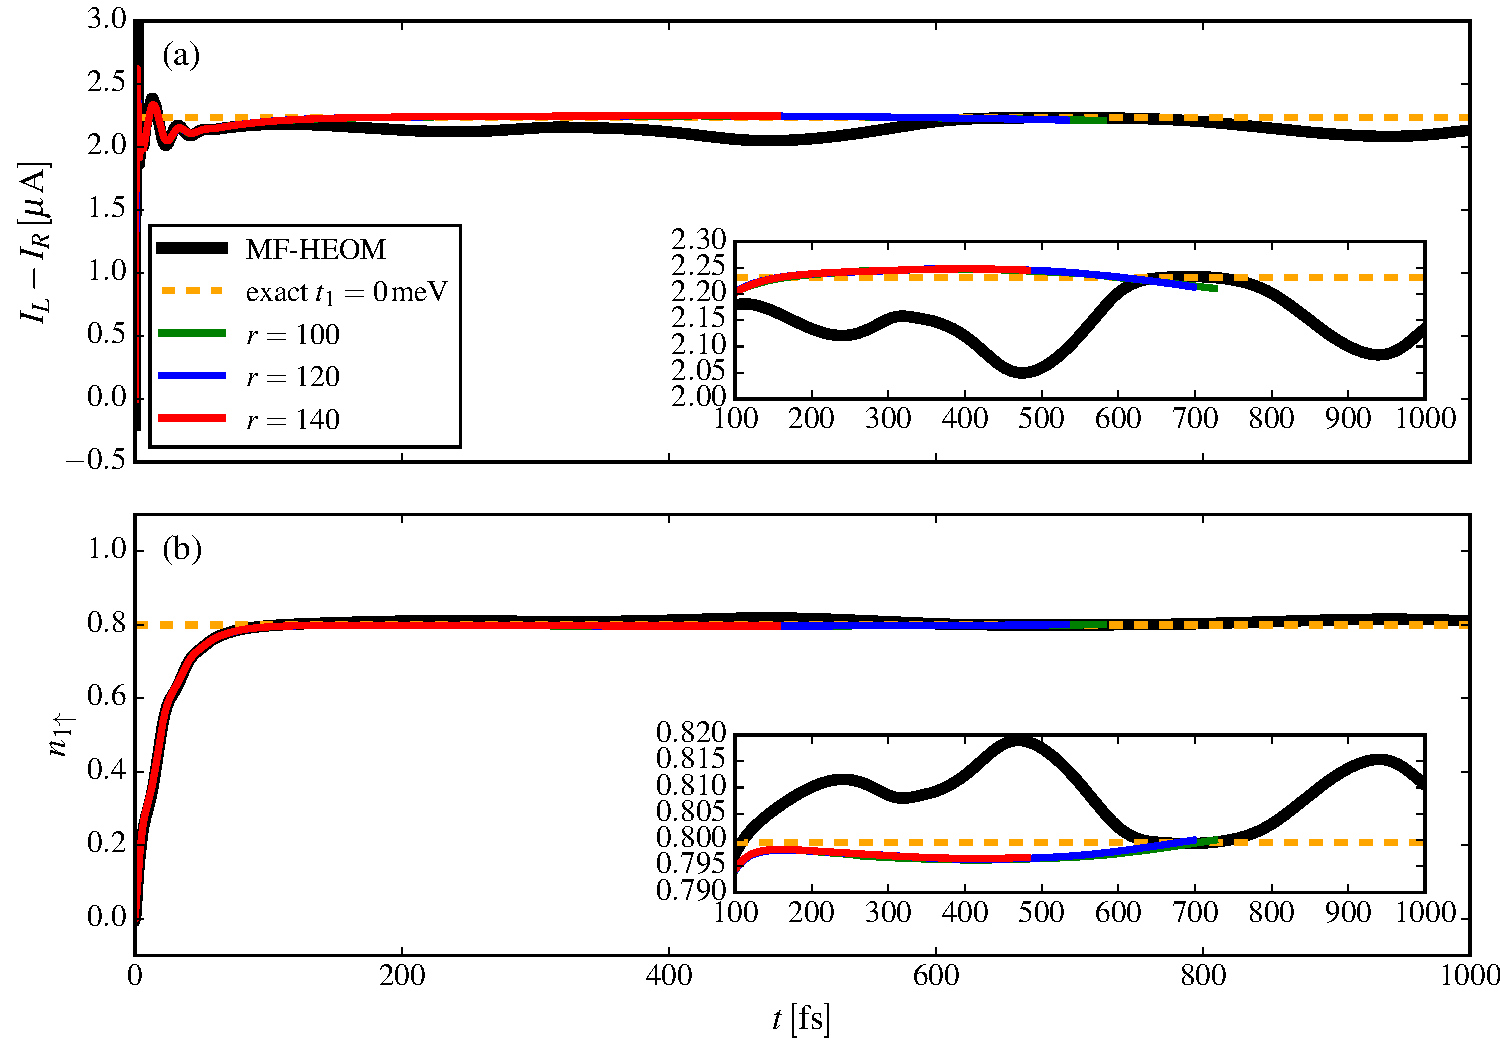
\includegraphics[width=0.9\textwidth]{figs/Comparison_TTHEOM_MFHEOM_Fransson_1x2_w0_0.05_V0.48_P0.5.pdf}
\end{figure}
\subsection{$P=0$}
\begin{figure}[!h]
	\centering
	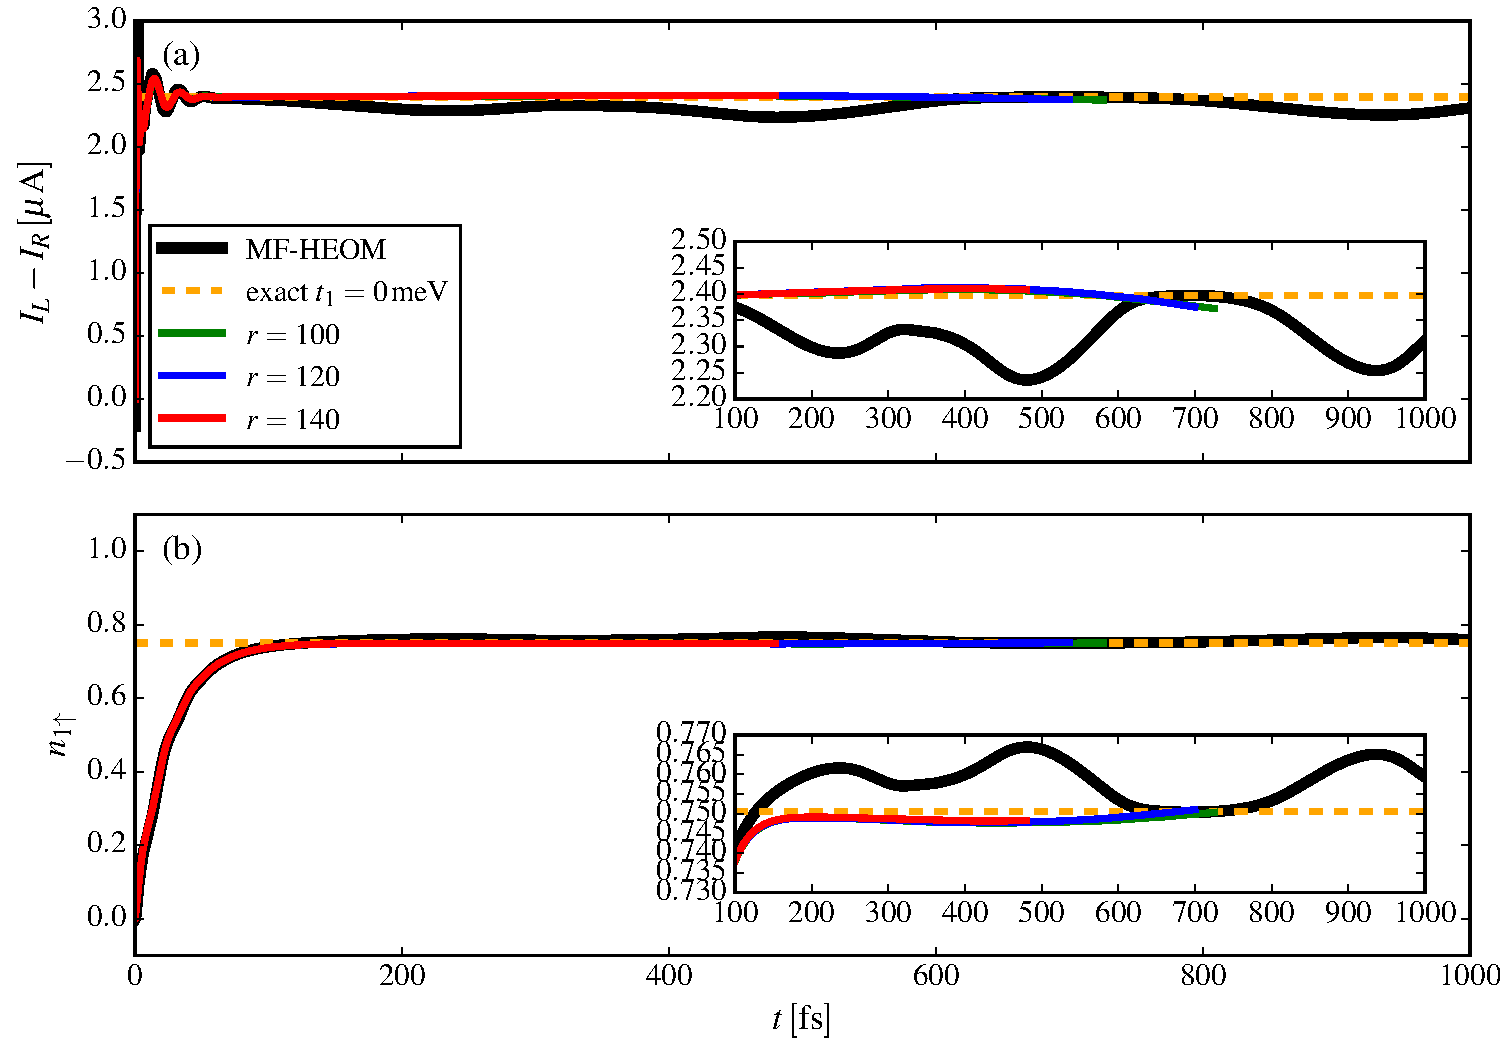
\includegraphics[width=0.9\textwidth]{figs/Comparison_TTHEOM_MFHEOM_Fransson_1x2_w0_0.05_V0.48_P0.0.pdf}
\end{figure}
\subsection{$P=-0.5$}
\begin{figure}[!h]
	\centering
	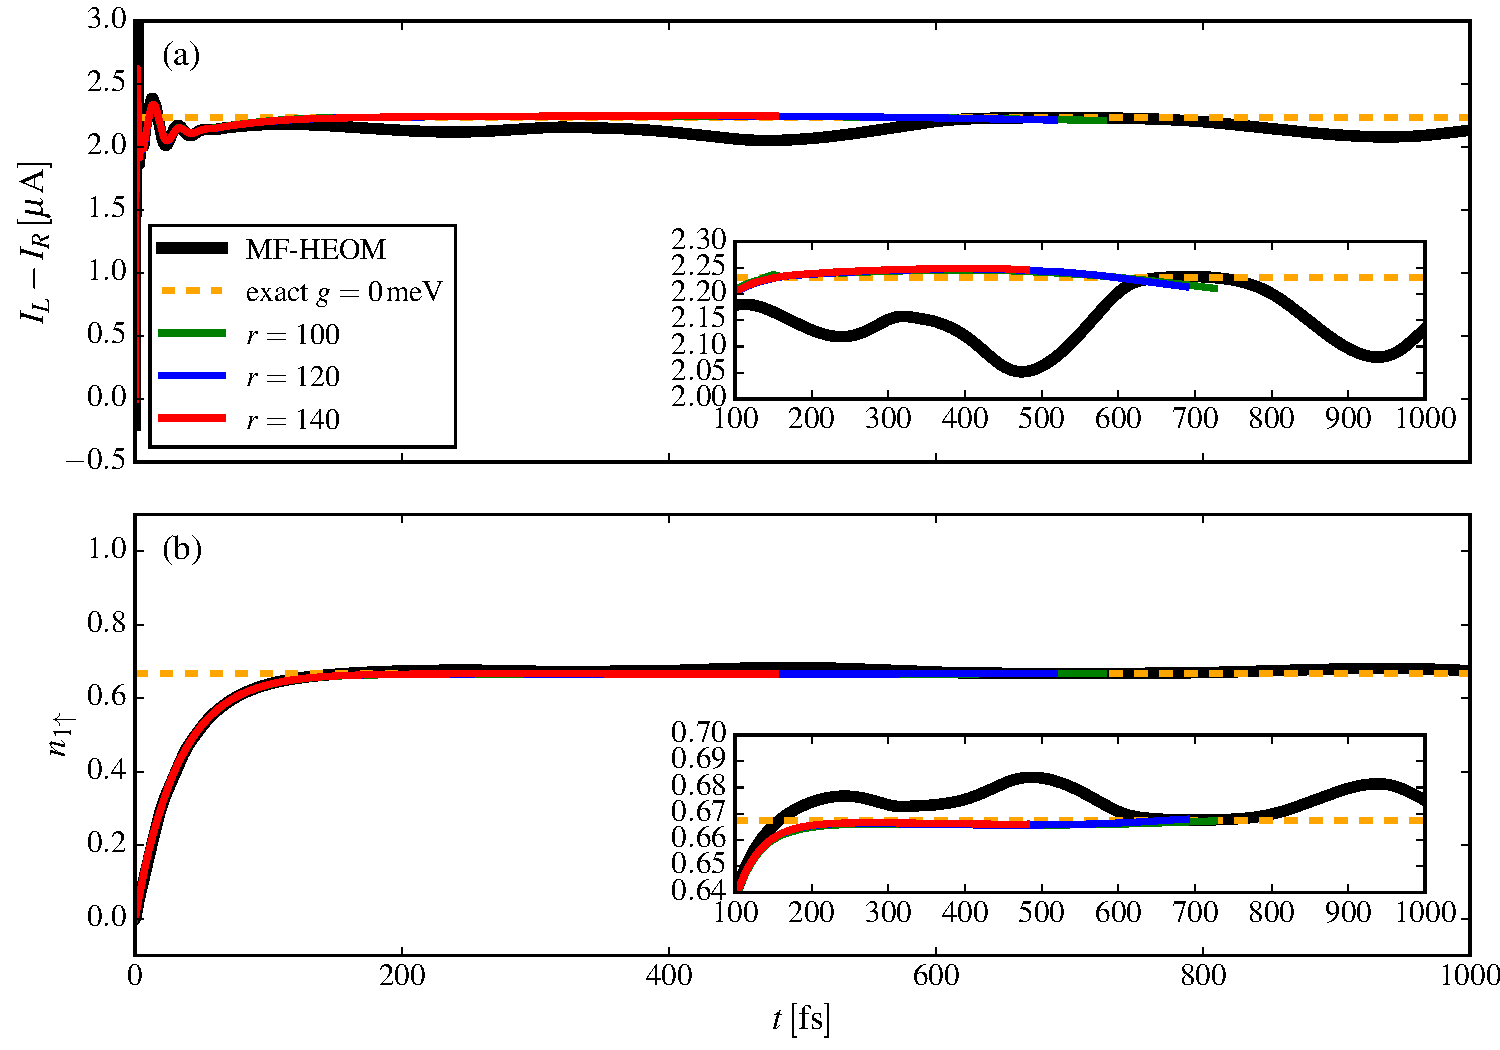
\includegraphics[width=0.9\textwidth]{figs/Comparison_TTHEOM_MFHEOM_Fransson_1x2_w0_0.05_V0.48_P-0.5.pdf}
\end{figure}
\section{$N=1\times 3$}
\section{$N=2\times 2$}
\end{document}




